\documentclass[ignorenonframetext,]{beamer}
\usetheme{Rochester}
%\usecolortheme{beaver}
\setbeamertemplate{caption}[numbered]
\setbeamertemplate{caption label separator}{:}
\setbeamercolor{caption name}{fg=normal text.fg}
\usepackage{amssymb,amsmath}
\usepackage{ifxetex,ifluatex}
\usepackage{fixltx2e} % provides \textsubscript
\usepackage{lmodern}
\ifxetex
  \usepackage{fontspec,xltxtra,xunicode}
  \defaultfontfeatures{Mapping=tex-text,Scale=MatchLowercase}
  \newcommand{\euro}{€}
\else
  \ifluatex
    \usepackage{fontspec}
    \defaultfontfeatures{Mapping=tex-text,Scale=MatchLowercase}
    \newcommand{\euro}{€}
  \else
    \usepackage[T1]{fontenc}
    \usepackage[utf8]{inputenc}
      \fi
\fi
% use upquote if available, for straight quotes in verbatim environments
\IfFileExists{upquote.sty}{\usepackage{upquote}}{}
% use microtype if available
\IfFileExists{microtype.sty}{\usepackage{microtype}}{}
\usepackage{graphicx}
\makeatletter
\def\maxwidth{\ifdim\Gin@nat@width>\linewidth\linewidth\else\Gin@nat@width\fi}
\def\maxheight{\ifdim\Gin@nat@height>\textheight0.8\textheight\else\Gin@nat@height\fi}
\makeatother
% Scale images if necessary, so that they will not overflow the page
% margins by default, and it is still possible to overwrite the defaults
% using explicit options in \includegraphics[width, height, ...]{}
\setkeys{Gin}{width=\maxwidth,height=\maxheight,keepaspectratio}

% Comment these out if you don't want a slide with just the
% part/section/subsection/subsubsection title:
\AtBeginPart{
  \let\insertpartnumber\relax
  \let\partname\relax
  \frame{\partpage}
}
% \AtBeginSection{
  % \let\insertsectionnumber\relax
  % \let\sectionname\relax
  % \frame{\sectionpage}
% }
% \AtBeginSubsection{
  % \let\insertsubsectionnumber\relax
  % \let\subsectionname\relax
  % \frame{\subsectionpage}
% }

\setlength{\parindent}{0pt}
\setlength{\parskip}{6pt plus 2pt minus 1pt}
\setlength{\emergencystretch}{3em}  % prevent overfull lines
\setcounter{secnumdepth}{0}
\usepackage[german]{babel}

\usepackage{hyperref}

\usepackage[absolute,overlay]{textpos}
\newcommand{\source}[1]{\begin{textblock*}{4cm}(8.7cm,8.6cm)
    \begin{beamercolorbox}[ht=0.5cm,right]{framesource}
        \usebeamerfont{framesource}\usebeamercolor[fg]{framesource} Quelle: {#1}
    \end{beamercolorbox}
\end{textblock*}}

\title{Die P $\neq$ NP-Vermutung}
\author{Adrian Hein, Florian Weber}
\date{6. Mai 2015}

\begin{document}
\frame{\titlepage}


\section{Motivation}
%\label{motivation}

\begin{frame}{Motivation}
	\begin{figure}
		\centering
		
\includegraphics{img/Comic1.png}\\
		{\small „I can't find an efficient algorithm, I guess I'm just to dumb.“}
	\end{figure}
\end{frame}

\begin{frame}{Motivation}
	\begin{figure}
		\centering
		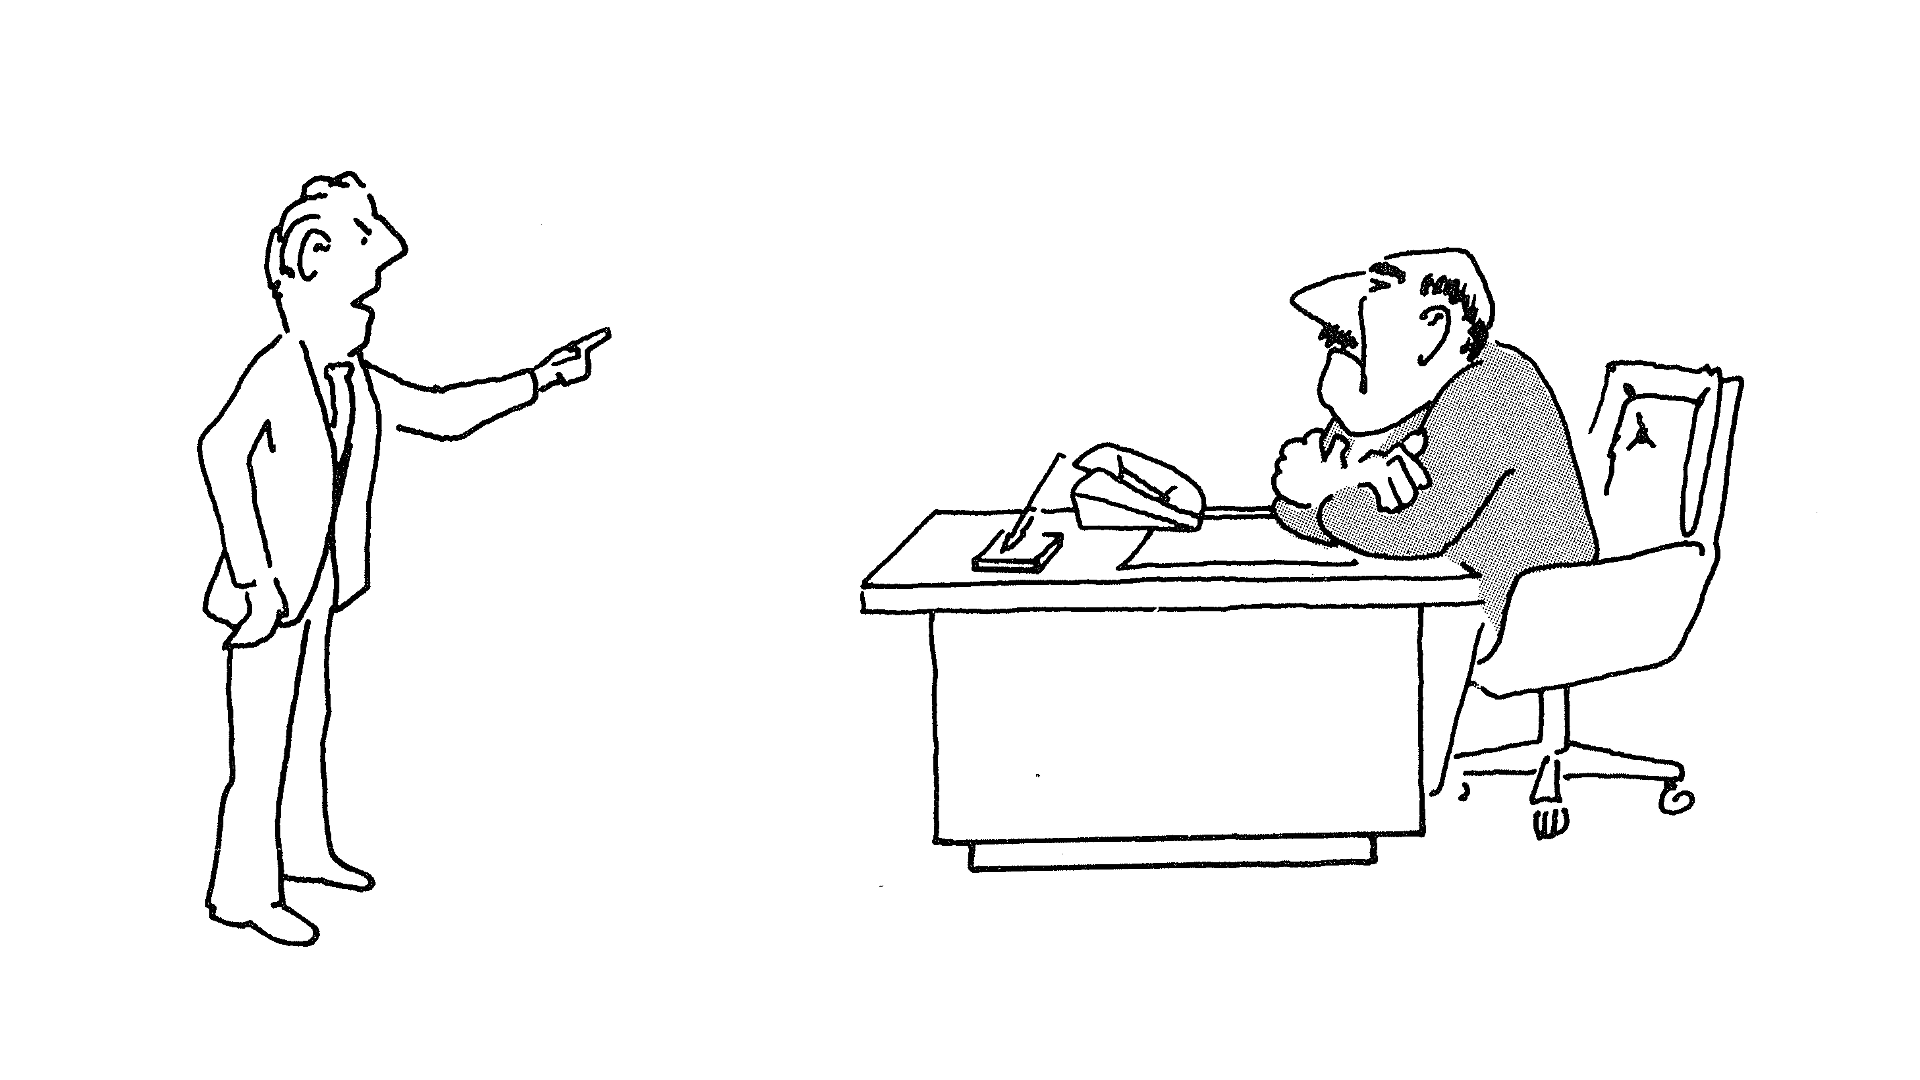
\includegraphics{img/Comic2.png}\\
		{\small „I can't find an efficient algorithm, because no such algorithm is possible.“}
	\end{figure}
\end{frame}

\begin{frame}{Motivation}
	\begin{figure}
		\centering
		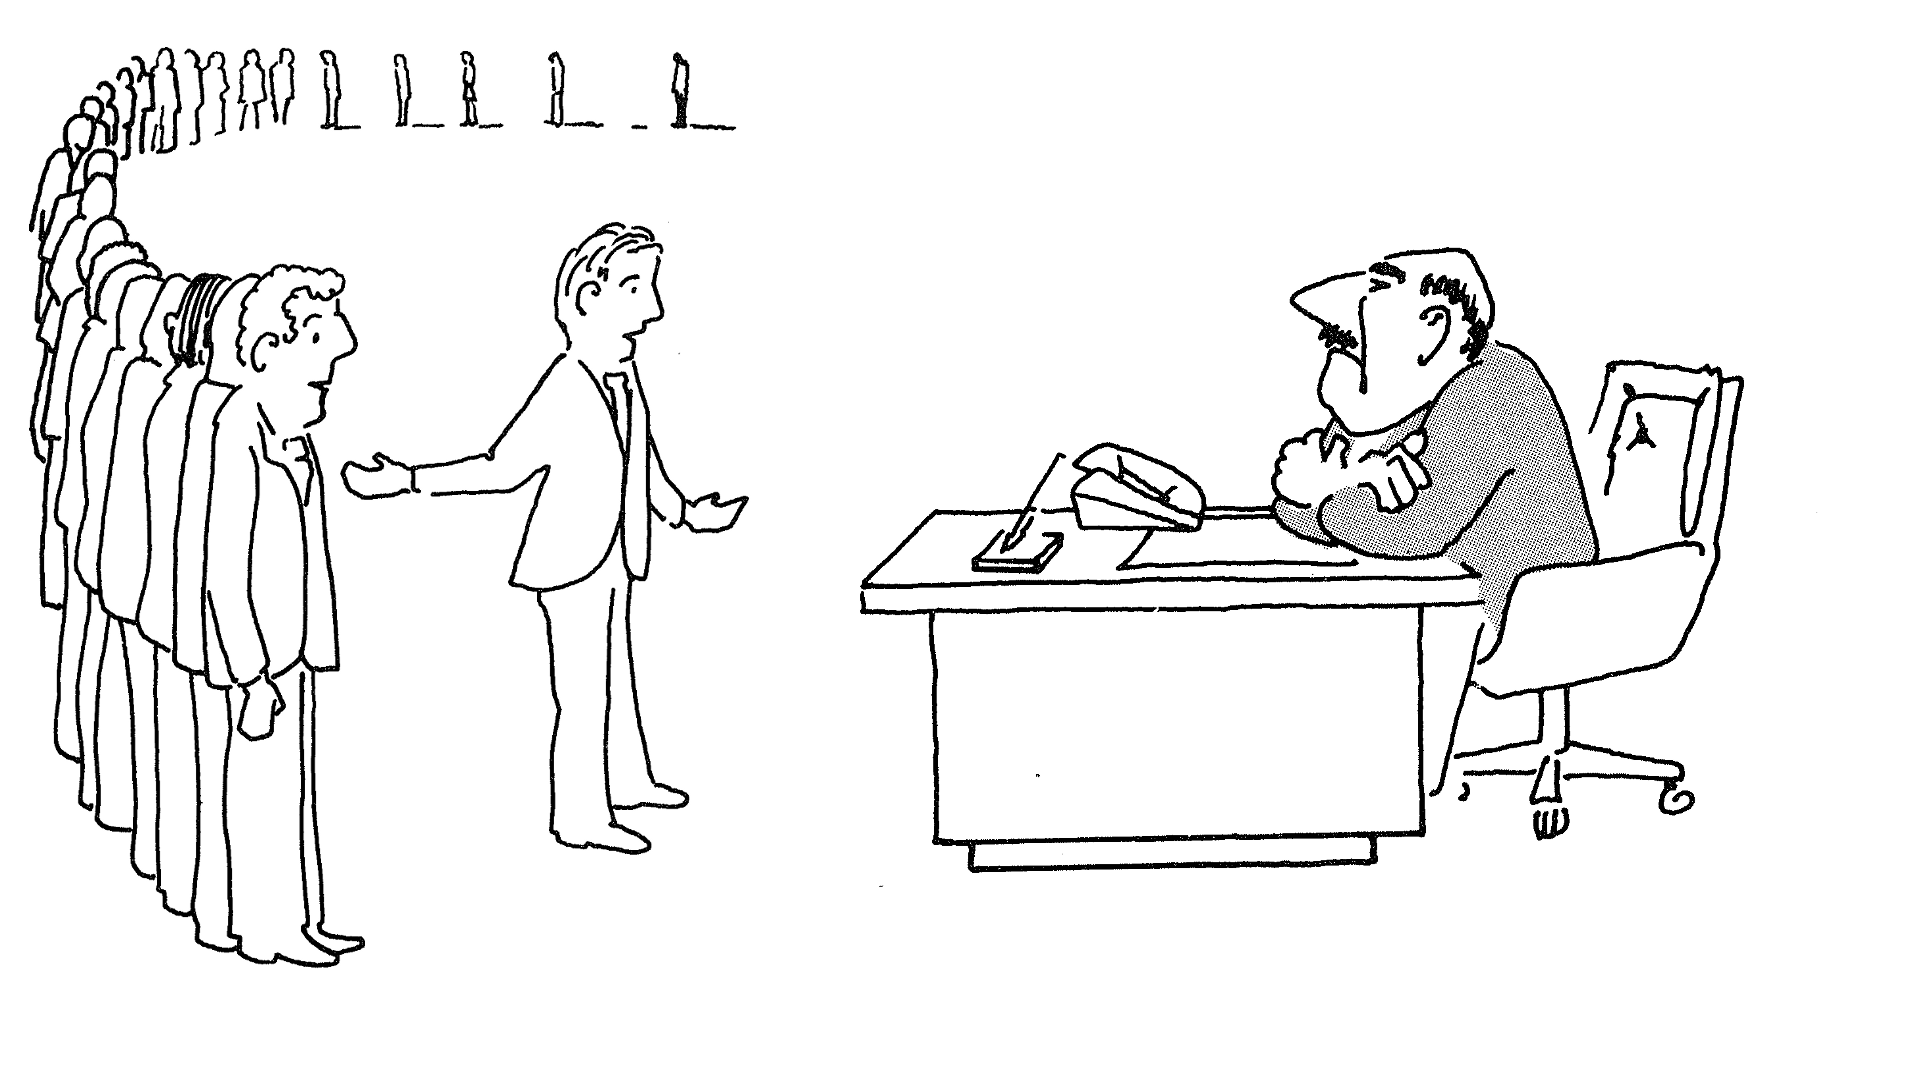
\includegraphics{img/Comic3.png}\\
		{\small „I can't find an efficient algorithm, but neither can all these famous people.“}
	\end{figure}
\end{frame}


\begin{frame}{Themen}
%\tableofcontents[hideallsubsections]
%Sadly the default TOC is horribly broken regarding vertical space, so let's do it by hand:
\begin{itemize}
	\item Einführung
	\item Das Cook-Levin Theorem
	\item Wichtige NP-vollständige Probleme
	\item Andere Komplexitätsklassen
	\item Indizien
	\item Implikationen
	\item Umgang mit NP-vollständigen Problemen
	\item Zusammenfassung
	\item Quellen
\end{itemize}
\end{frame}


\section{Einführung}\label{einfuxfchrung}

\begin{frame}{Einführung}{Turingmaschine}
\begin{itemize}
\itemsep1pt\parskip0pt\parsep0pt
\item
  Mathematische Abstraktion eines Computers
\item
  Besteht aus:

  \begin{itemize}
  \itemsep1pt\parskip0pt\parsep0pt
  \item
    Steuerwerk
  \item
    unendlich langes Steuerband
  \item
    Lese- und Schreibkopf
  \end{itemize}
\end{itemize}

\end{frame}

\begin{frame}{Einführung}{Turingmaschine}

\begin{itemize}
\itemsep1pt\parskip0pt\parsep0pt
\item
  Pro Schritt wird:

  \begin{itemize}
  \itemsep1pt\parskip0pt\parsep0pt
  \item
    ein Zeichen gelesen
  \item
    ein Zeichen geschrieben
  \item
    eine Bewegung ausgeführt
  \end{itemize}
\item
  Jeder Schritt ist nur abhängig von:

  \begin{itemize}
  \itemsep1pt\parskip0pt\parsep0pt
  \item
    aktuellem Zeichen auf dem Band
  \item
    aktuellem Zustand der TM
  \end{itemize}
\item
  Eine TM hat endlich viele Zustände
\item
  Man kann Zustände als Endzustände definieren
\end{itemize}

\end{frame}

\begin{frame}{Einführung}{Turingmaschine}

\begin{figure}[htbp]
\centering
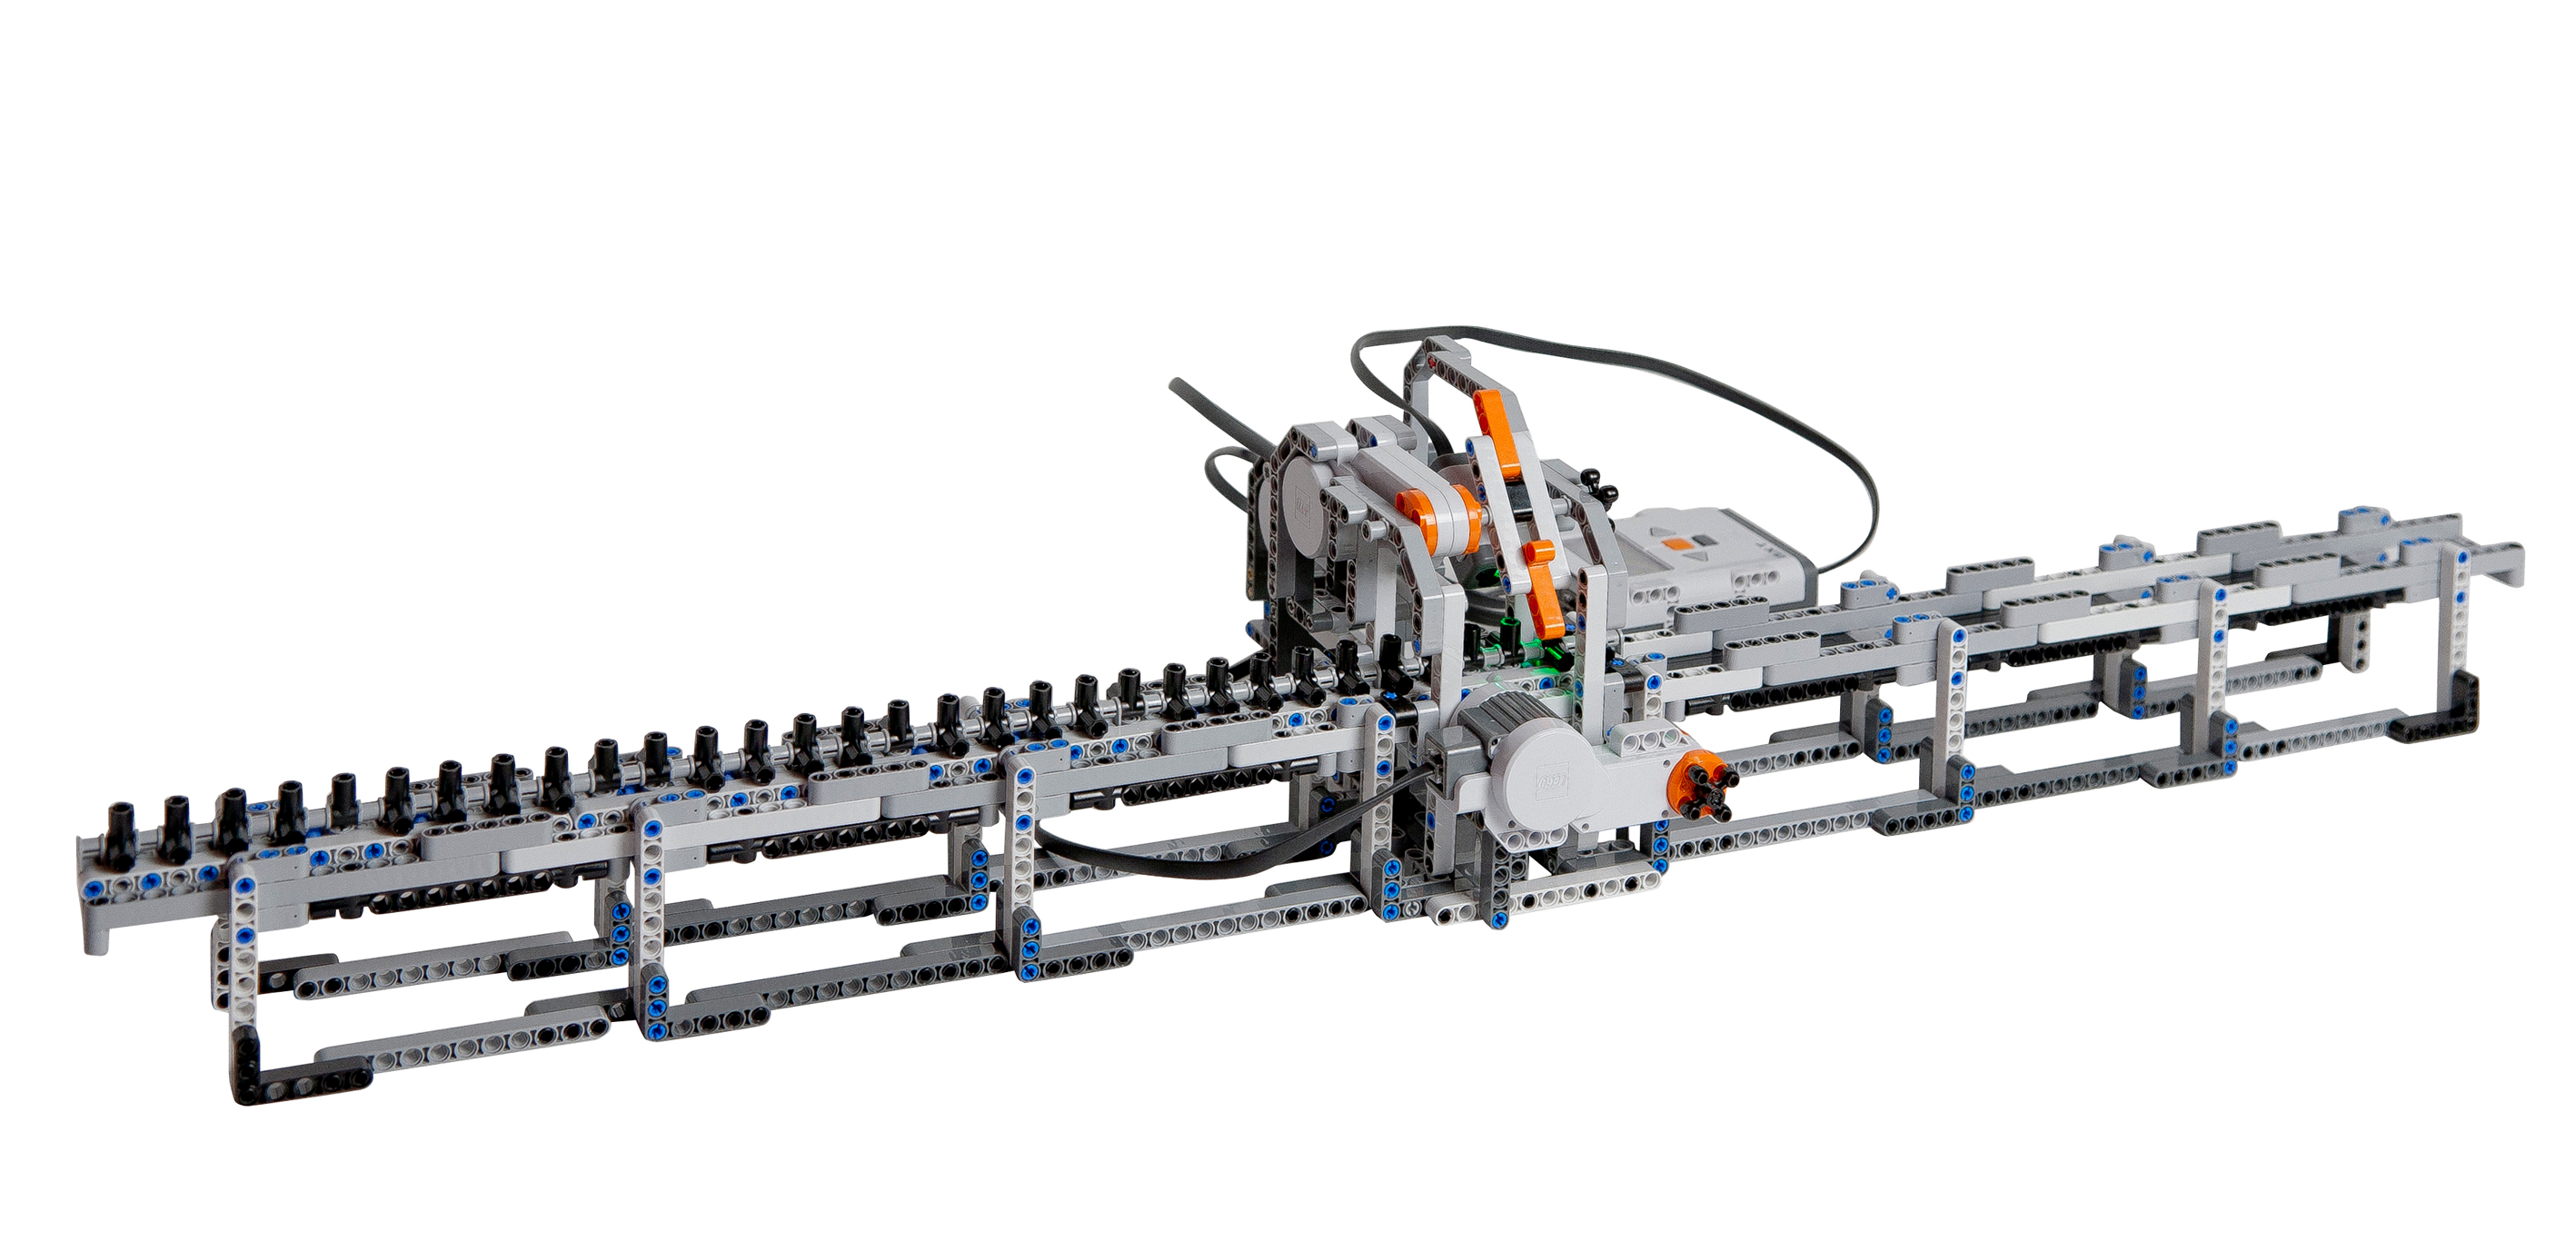
\includegraphics{img/lego_tm.png}

\end{figure}

\end{frame}

\begin{frame}{Einführung}{Turingmaschine formal}

\begin{itemize}
\itemsep1pt\parskip0pt\parsep0pt
\item
  Formal besteht eine TM aus einem Tupel
  $\mathcal{M}:=\{ Q, \Sigma, \Gamma, \delta, q_0, F \}$ mit:

  \begin{itemize}
  \itemsep1pt\parskip0pt\parsep0pt
  \item
    $Q$, der endlichen Zustandsmenge
  \item
    $\Sigma$, dem endlichen Eingabealphabet
  \item
    $\Gamma$, dem endliche Bandalphabet und es gilt
    $\Sigma \subset \Gamma$
  \item
    $\delta\colon (Q \setminus F)\times \Gamma \to Q \times \Gamma \times \{L, 0, R\}$,
    der (partiellen) Überführungsfunktion
  \item
    $q_0 \in Q$, dem Anfangszustand
  \item
    $F \subseteq Q$, der Menge der akzeptierenden Zustände
  \end{itemize}
  \item
    $\square \in \Gamma\setminus\Sigma$ bezeichnet das leere Feld
\end{itemize}

\end{frame}

\begin{frame}{Einführung}{Turingmaschine (nichtdeterministisch)}

\begin{itemize}
\itemsep1pt\parskip0pt\parsep0pt
\item
  Ähnlich der deterministischen TM
\item
  NDTM hat allerdings mehrere Übergangsfunktionen
\item
  Endet eine Sequenz von Entscheidungen in $F$ gilt die Eingabe als
  akzeptiert
\item
  Im Gegensatz zur deterministischen TM nicht ohne Weiteres realisierbar
\end{itemize}

\end{frame}

\begin{frame}{Einführung}{Turingmaschine (Mehrband)}

\begin{itemize}
\itemsep1pt\parskip0pt\parsep0pt
\item
  Hat anstatt einem Band mehrere mit jeweils einem Lese- und
  Schreibkopf\\
\begin{figure}[htbp]
\begin{minipage}{0.4\textwidth}
\centering
\scalebox{0.65}{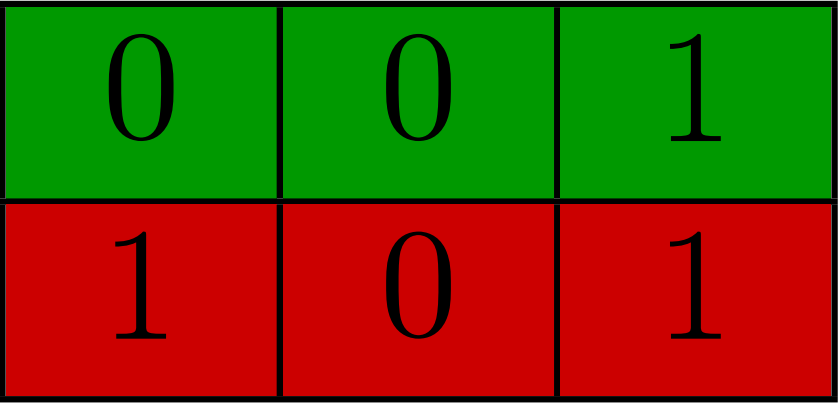
\includegraphics{img/TM0.png}}
\end{minipage}
\begin{minipage}{0.1\textwidth}
\centering
$\Rightarrow$
\end{minipage}
\begin{minipage}{0.4\textwidth}
\centering
\scalebox{0.7}{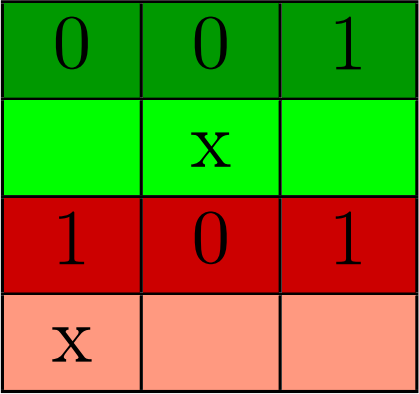
\includegraphics{img/TM1.png}}
\end{minipage}
\end{figure}

\item
  Kann durch eine TM mit einem Band simuliert
  werden\\
\item[]
\scalebox{0.7}{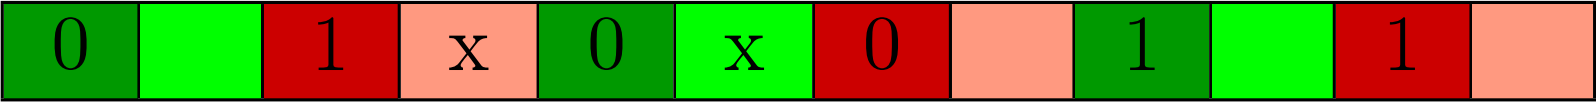
\includegraphics{img/TM2.png}}

\item
  Mehrband TMs sind genauso mächtig wie normale TMs aber evt.
  anschaulicher
\end{itemize}

\end{frame}

\begin{frame}{Einführung}{Die Klasse P}

\begin{itemize}
\itemsep1pt\parskip0pt\parsep0pt
\item
  Enthält alle Entscheidungsprobleme die in Polynomialzeit von einer TM
  lösbar sind
\item
  Probleme in P gelten als praktisch lösbar
\item
  Ist unter Komplementbildung abgeschlossen
\item
  Beispiele sind:

  \begin{itemize}
  \itemsep1pt\parskip0pt\parsep0pt
  \item
    Lineare Programmierung/Optimierung
  \item
    PRIMES (AKS-Primzahltest)
  \item
    SET-COVER
  \end{itemize}
\end{itemize}

\end{frame}

\begin{frame}{Einführung}{Die Klasse NP (formal)}

\begin{itemize}
\itemsep1pt\parskip0pt\parsep0pt
\item
  Eine Sprache $L \subseteq \{0, 1\}^*$ liegt in NP, wenn es:

  \begin{itemize}
  \itemsep1pt\parskip0pt\parsep0pt
  \item
    ein Polynom $p: \mathbb{N} \rightarrow \mathbb{N}$
  \item
    sowie eine in Polynomialzeit laufende TM $\mathcal{M}$, den
    sogenannten Verifizierer für $L$, gibt
  \item
    sodass für jedes $x \in \{0, 1\}^*$ gilt:

    \begin{itemize}
    \itemsep1pt\parskip0pt\parsep0pt
    \item
      $x \in L \Leftrightarrow \exists u \in \{0, 1\}^{p(|x|)}$, sodass
      $\mathcal{M}(x, u) = 1$
    \end{itemize}
  \end{itemize}
\item
  In diesem Fall nennt man $u$ ein Zertifikat für $x$.
\end{itemize}

\end{frame}

\begin{frame}{Einführung}{Die Klasse NP (alternativ)}

\begin{itemize}
\itemsep1pt\parskip0pt\parsep0pt
\item
  Alle Entscheidungsprobleme die von einer NDTM $\mathcal{M}$ in
  Polynomialzeit gelöst werden
\item
  $x$ ist eine Lösung, wenn es eine Sequenz von Entscheidungen gibt,
  sodass $\mathcal{M}$ in einem der aktzeptierenden Zustände ($F$) hält.

\item
  Ursprüngliche Definition, deswegen auch NP (nondeterministic
  polynomial time)
\item
  Beide Definitionen äquivalent, da die Sequenz von Entscheidungen, die
  zu $F$ führt als Zertifikat betrachtet werden kann
\end{itemize}

\end{frame}

\begin{frame}{Einführung}{Die Klasse coNP}

\begin{itemize}
\itemsep1pt\parskip0pt\parsep0pt
\item
  Alle Sprachen, deren Komplement in NP liegt
\item
  NICHT das Komplement zu NP
\item
  Beispiel: Kontradiktion
\end{itemize}

\end{frame}

\begin{frame}{Einführung}{Reduktion}

\begin{itemize}
\itemsep1pt\parskip0pt\parsep0pt
\item
  $A$ heißt reduzierbar auf $B$, wenn es einen Algorithmus gibt, der aus
  jedem Problem aus $A$ in Polynomialzeit ein Problem aus $B$ macht
\item
  Man schreibt dann $A \preceq B$
\item
  Gibt es einen Algorithmus zur Lösung von $B$ und gilt $A \preceq B$,
  so kann dieser auch $A$ lösen
\item
  Man sagt $B$ ist mindestens so schwer wie $A$
\end{itemize}

\end{frame}

\begin{frame}{Einführung}{NP-Vollständigkeit}

\begin{itemize}
\itemsep1pt\parskip0pt\parsep0pt
\item
  Gilt $L \preceq L',\ \forall L \in$ NP, so nennt man $L'$ NP-schwer
\item
  Liegt $L'$ selber auch in NP nennt man $L'$ NP-vollständig
\item
  Um NP-schwere für $L'$ zu zeigen genügt es $L \preceq L'$ für ein
  NP-schweres $L$ zu zeigen
\item
  Ist ein Problem $A$ NP-schwer, so ist das entsprechende Problem
  $\overline{A}$ in coNP logischerweise coNP-schwer
\end{itemize}

\end{frame}

\section{Cook-Levin Theorem}\label{cook-levin-theorem}

\begin{frame}{Das Cook-Levin Theorem}

\begin{figure}[htbp]
\centering
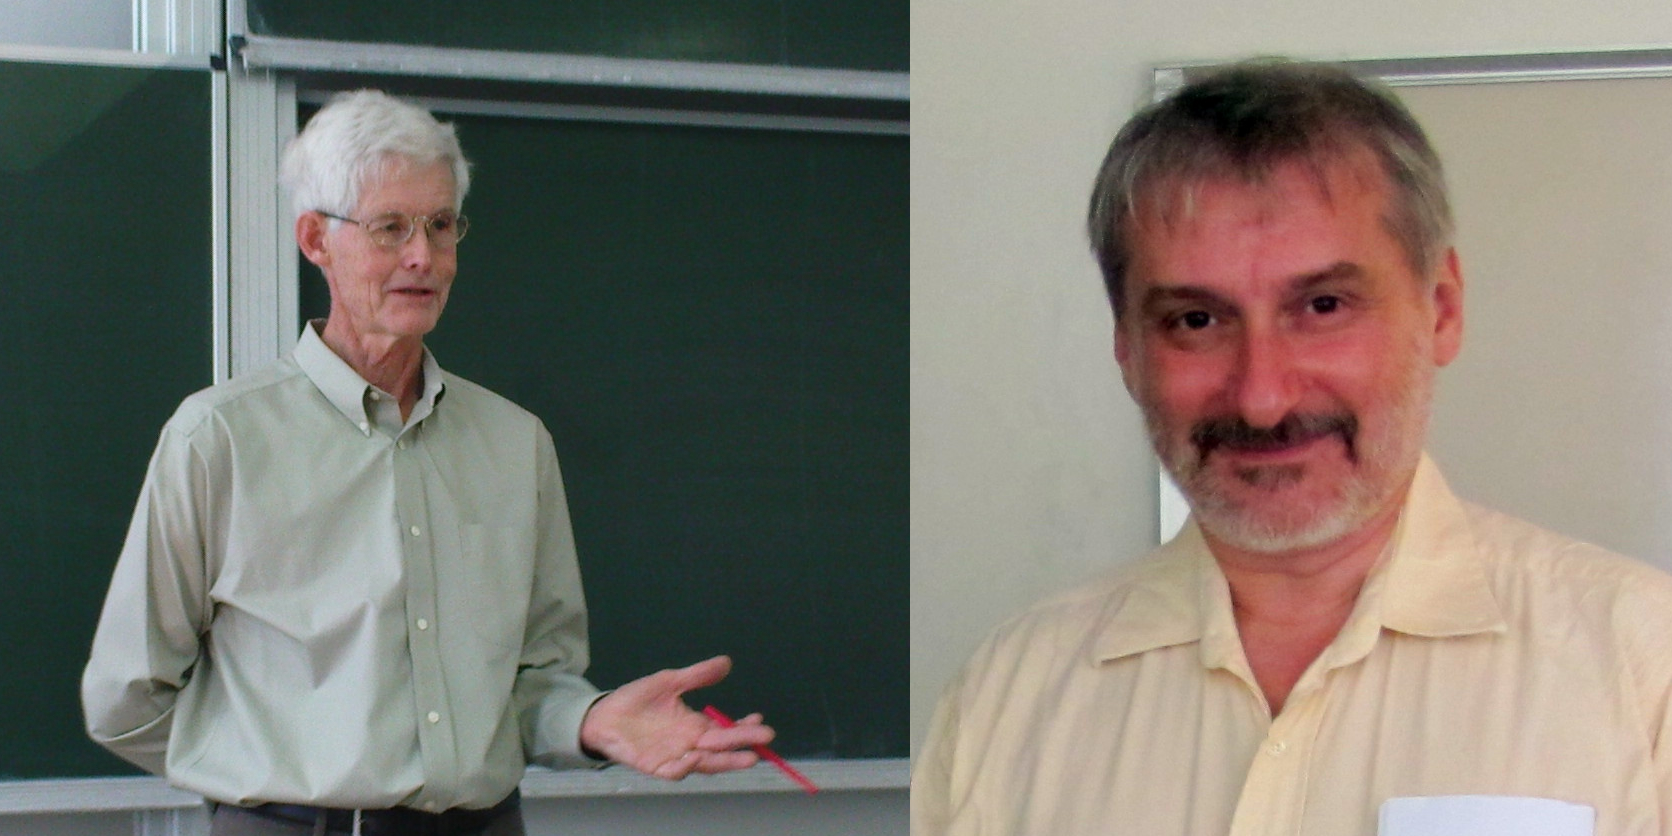
\includegraphics{img/cook_levin.png}\\

Stephen Cook, Leonid Levin
\end{figure}

\end{frame}

\begin{frame}{Das Cook-Levin Theorem}{Konjunktive Normalform}

\begin{itemize}
\itemsep1pt\parskip0pt\parsep0pt
\item
  Boolsche Funktionen der Form
  \[(a \vee b \vee c) \wedge (d \vee e) \wedge (f \vee g \vee h \vee i)\]
  stehen in \textbf{konjunktiver Normalform}
\item
  Lösungen stellen alle Belegungen dar, die zu 1 evaluieren
\item
  Das Entscheidungsproblem, ob es eine Lösung gibt, ist als \textbf{SAT}
  (von „satisfiable``) bekannt
\item
  Der Spezialfall, bei dem jede Teilklausel genau drei Variablen
  beinhaltet, heißt \textbf{3SAT}:
  \[(a \vee b \vee c) \wedge (d \vee e \vee f) \wedge \dots\]
\end{itemize}

\end{frame}

\begin{frame}{Das Cook-Levin Theorem}{Boolsche Funktionen}

\begin{itemize}
\itemsep1pt\parskip0pt\parsep0pt
\item
  Jede boolsche Funktion lässt sich in konjunktiver Normalform
  darstellen
\item
  TMs die Sprachen entscheiden, sind boolsche Funktionen
\item
  Die Größe einer KNF für $n$ Variablen liegt in $O(n \cdot 2^n)$
\end{itemize}

\end{frame}

\begin{frame}{Das Cook-Levin Theorem}{Reduktion * auf SAT}

\begin{itemize}
\itemsep1pt\parskip0pt\parsep0pt
\item
  $O(n \cdot 2^n)$ offensichtlich zu groß
\item
  Sei $\mathcal{M}$ eine TM die eine NP-vollständige Sprache entscheidet
  und die

  \begin{itemize}
  \itemsep1pt\parskip0pt\parsep0pt
  \item
    ein Eingabe- und ein Ausgabe/Arbeitsband habe
  \item
    bei der die Position des Kopfes in Schritt $i$ nur von der Länge der
    Eingabe abhängt
  \item
    gültige Annahme, da in $O(f(n)^2)$ simulierbar
  \end{itemize}
\item
  Sei $Q$ die Menge der Zustände von $\mathcal{M}$
\item
  Sei $\Gamma$ das Bandalphabet von $\mathcal{M}$
\item
  Sei $\langle a, b, q\rangle_i \in \Gamma\times \Gamma\times Q$ der
  Snapshot von $\mathcal{M}$ in Schritt $i$
\end{itemize}

\end{frame}

\begin{frame}{Das Cook-Levin Theorem}{Reduktion * auf SAT}

\begin{itemize}
\itemsep1pt\parskip0pt\parsep0pt
\item
  Snapshots können offensichtlich als Zeichenketten konstanter Länge
  kodiert werden.
\item
  Ein Snapshot $S_i$ hängt ab von:

  \begin{itemize}
  \itemsep1pt\parskip0pt\parsep0pt
  \item
    $S_{i-1}$
  \item
    einem Zeichen fester Position der Eingabe
  \item
    dem letzten Snapshot an der selben Stelle
  \end{itemize}
\item
  Es gibt für jedes $i$ genau einen korrekten Snapshot
\item
  Daraus folgt: Es gibt eine Funktion $f$, die zwei Snapshots und eine
  Position auf dem Eingabeband auf einen neuen Snapshot abbilden:
  \[S_i = f(S_{i-1}, S_{\mathrm{prev}(i)}, E_{\mathrm{inputpos}(i)})\]
\end{itemize}

\end{frame}

\begin{frame}{Das Cook-Levin Theorem}{Reduktion * auf SAT}

\begin{itemize}
\itemsep1pt\parskip0pt\parsep0pt
\item
  Um eine Lösung für die betrachtete Sprache zu finden, muss man eine
  Abfolge von TM-Schritten finden, die zum Ergebnis führt.
\item
  Die einzelnen Schritte (und damit die Snapshotkette) kodieren eine
  Lösung, sind aber zunächst unbekannt.
\item
  Die Snapshotkette lässt sich aber als polynomielle KNF schreiben.
\item
  Angenommen, es gäbe einen Polyzeit-Entscheider für SAT, so könnte
  dieser damit auch die Kette von Snapshots für andere Probleme finden,
  und damit diese in Polyzeit entscheiden!
\end{itemize}

\end{frame}

\begin{frame}{Das Cook-Levin Theorem}{Reduktion SAT auf 3SAT}

\begin{itemize}
\itemsep1pt\parskip0pt\parsep0pt
\item
  Wir möchten die Klausel $F_1 = (a \vee b \vee c \vee d)$ mit Lösung
  $L_1$ in 3SAT-Klauseln zerlegen
\item
  Sei $h$ eine neu eingeführte Hilfsvariable
\item
  Dann ist $F_2 = (a \vee b \vee h) \wedge (\overline{h} \vee c \vee d)$
  mit Lösung $L_2$ eine äquivalente Formel
\item
  Erfüllbarkeit ist äquivalent:

  \begin{itemize}
  \itemsep1pt\parskip0pt\parsep0pt
  \item
    $F_1 \Rightarrow F_2$: 2 Fälle:

    \begin{itemize}
    \itemsep1pt\parskip0pt\parsep0pt
    \item
      $a \vee b = 1$: $L_2$ mit $h = 0$ erfüllt
    \item
      $c \vee d = 1$: $L_2$ mit $h = 1$ erfüllt
    \end{itemize}
  \item
    $F_2 \Rightarrow F_1$: 2 Fälle:

    \begin{itemize}
    \itemsep1pt\parskip0pt\parsep0pt
    \item
      $h = 0 \Rightarrow (a \vee b) = 1$
    \item
      $h = 1 \Rightarrow (c \vee d) = 1$
    \end{itemize}
  \end{itemize}
\end{itemize}

\end{frame}

\begin{frame}{Das Cook-Levin Theorem}{Reduktion SAT auf 3SAT}

\begin{itemize}
\itemsep1pt\parskip0pt\parsep0pt
\item
  Allgemein gilt: Um eine SAT-Klausel
  $(a_1 \vee a_2 \vee \dots \vee a_n)$ nach 3SAT zu konvertieren, genügt
  es, sie wie folgt zu schreiben:
  \[ (a_1 \vee a_2 \vee h_1) \wedge (\overline{h_1} \vee a_3 \vee h_2) \wedge \dots \wedge (\overline{h_{n-2}} \vee a_{n-1} \vee a_n) \]
\item
  $h_1 \dots h_{n-2}$ sind hierbei neu eingeführte Hilfsvariablen
\item
  SAT liegt in NP $\Rightarrow$ 3SAT liegt als Spezialfall von SAT in NP
\item
  Laufzeit der Reduktion SAT $\rightarrow$ 3SAT ist polynomiell 
\item
  $\Rightarrow$ 3SAT ist NP-vollständig
\end{itemize}

\end{frame}

\section[Probleme]{Wichtige NP-vollständige Probleme}

\begin{frame}{Wichtige NP-vollständige Probleme}

\begin{figure}[htbp]
\centering
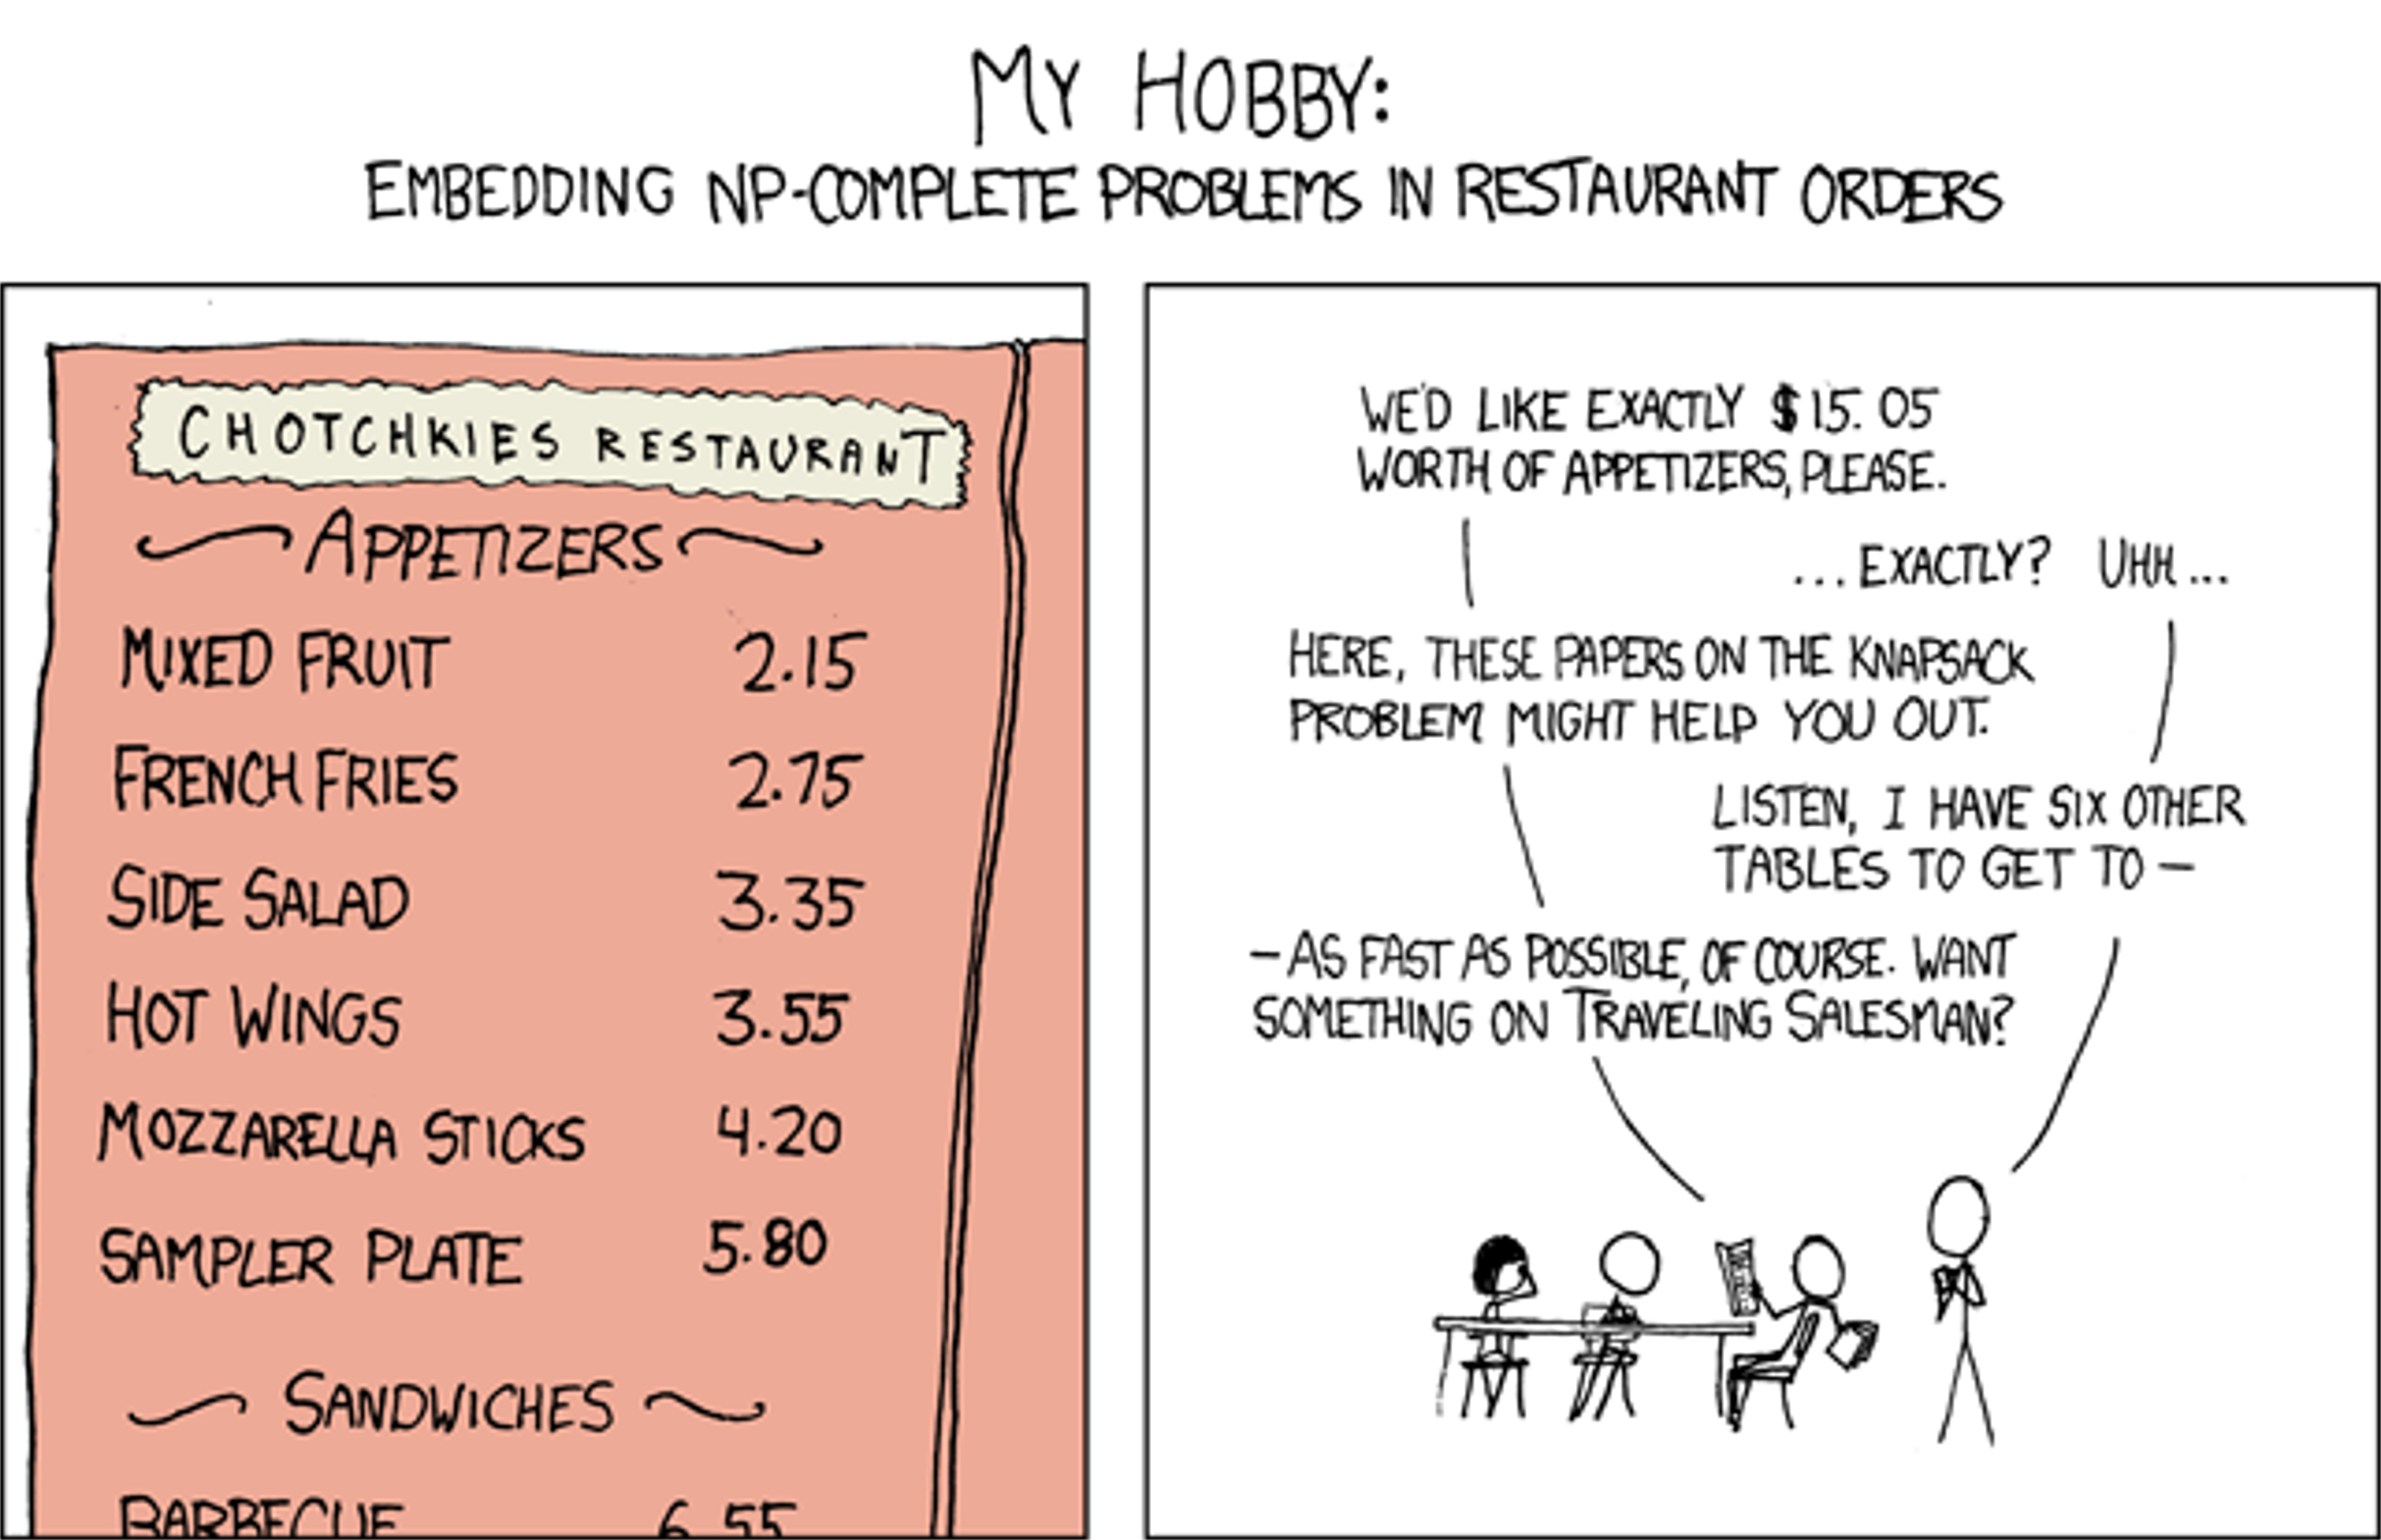
\includegraphics{img/xkcd_np_complete_big.png}
\end{figure}

\end{frame}

\begin{frame}{Wichtige NP-vollständige Probleme}{INDSET}

\begin{quote}
	Besitzt ein Graph $G$ mindestens $k$ paarweise nicht über eine Kante
verbundene Knoten (=stabile Menge)?
\end{quote}

INDSET ist NP-vollständig. Hierzu definieren wir eine Transformation
beliebiger 3SAT-Instanzen zu Graphen:

\begin{itemize}
\itemsep1pt\parskip0pt\parsep0pt
\item
  Erzeuge für jede Klausel einen vollständig verbundenen Teilgraph
  (=Clique), dessen Knoten jeweils eine gültige Belegung repräsentieren.
\item
  Verbinde alle nicht verbundenen Knoten, die gemeinsam zu einer
  widersprüchlichen Belegung führen würden.
\item
  Bestimme nun eine stabile Menge der Größe $k$. Deren Knoten kodieren
  nun eine gültige Belegung für die 3SAT-Instanz.
\end{itemize}

\end{frame}

\begin{frame}{Wichtige NP-vollständige Probleme}{0/1 IPROG}

\begin{itemize}
\itemsep1pt\parskip0pt\parsep0pt
\item
  Gegeben: $m$ lineare Ungleichungen über $n$ Variablen
\item
  Gesucht: eine Lösung für das System wobei die Variablen nur 0 oder 1
  annehmen können
\item
  In NP: die Belegung der Variablen kann als Zertifikat gesehen werden
\item
  NP-vollständig: SAT $\preceq$ 0/1 IPROG, da jede Klausel als
  Ungleichung aufgefasst werden kann

  \begin{itemize}
  \itemsep1pt\parskip0pt\parsep0pt
  \item
    $u_1 \vee \overline{u_2} \vee \overline{u_3}$ kann ausgedrückt
    werden durch $u_1 + (1 - u_2) + (1 - u_3) \geq 1$
  \end{itemize}
\end{itemize}
\end{frame}


\begin{frame}{Wichtige NP-vollständige Probleme}{Traveling Salesman (TSP)}

\begin{figure}[htbp]
\begin{minipage}{0.58\textwidth}
\begin{quote}
Gibt es zu $n$ Städten einen Rundweg der kürzer ist als $b$?
\end{quote}
\end{minipage}
\begin{minipage}{0.4\textwidth}
\centering
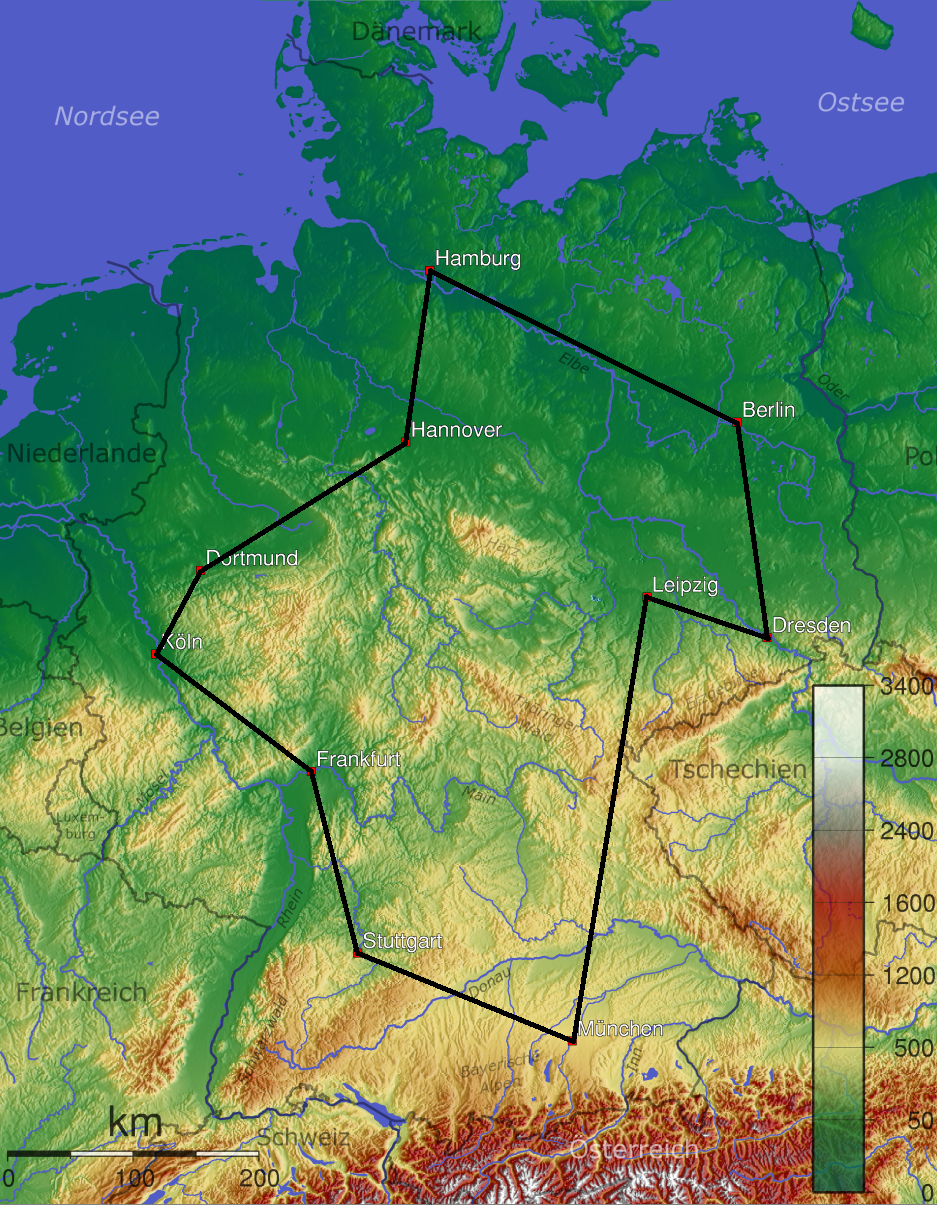
\includegraphics{img/tsp.png}
\end{minipage}
\end{figure}
\end{frame}

\section{Andere Klassen}\label{andere-klassen}

\begin{frame}{Andere Klassen}{NP-Intermediate}
\begin{itemize}
\itemsep1pt\parskip0pt\parsep0pt
\item
  Gilt P $\neq$ NP so gibt es eine Klasse NP-Intermediate (NPI) für die
  gilt:

  \begin{itemize}
  \itemsep1pt\parskip0pt\parsep0pt
  \item
    $A \in$ NPI $\Leftrightarrow A \in$ NP, $A \notin$ P und $A$ ist
    nicht NP-Schwer
  \end{itemize}
\item
  Wurde von Richard Ladner 1975 bewiesen
\item
  Er konstruierte ein künstliches Problem welches unter der Annahme P
  $\neq$ NP in NPI liegt
\item
  Es ist nicht sicher ob es ``natürliche'' Probleme in NPI gibt
\end{itemize}
\end{frame}

\begin{frame}{Andere Klassen}{Vermutete Probleme in NPI}
\begin{itemize}
\itemsep1pt\parskip0pt\parsep0pt
\item
  Man vermutet, dass die Primfaktorzerlegung in NPI liegt
\item
  Bisher noch kein Algorithmus in Polynomialzeit gefunden
\item
  Noch kein Beweis für NP-Schwere
\item
  Aktuelle Kryptographie baut darauf auf (RSA)
\end{itemize}
\end{frame}



\begin{frame}{Andere Klassen}{EXP und NEXP}

\begin{itemize}
\itemsep1pt\parskip0pt\parsep0pt
\item
  Probleme deren Zertifikat in exponentieller Zeit verfiziert bzw.
  gefunden werden kann.
\item
  In vieler Hinsicht analog zu P und NP, aber in der Praxis weniger
  interessant.
\end{itemize}

\end{frame}

\begin{frame}{Andere Klassen}{Platzbasierte}

\begin{itemize}
\itemsep1pt\parskip0pt\parsep0pt
\item
  L $\subseteq$ NL

  \begin{itemize}
  \itemsep1pt\parskip0pt\parsep0pt
  \item
    logarithmischer Platz
  \end{itemize}
\item
  PSPACE = NPSPACE

  \begin{itemize}
  \itemsep1pt\parskip0pt\parsep0pt
  \item
    polynomieller Platz
  \end{itemize}
\item
  EXPSPACE = NEXPSPACE

  \begin{itemize}
  \itemsep1pt\parskip0pt\parsep0pt
  \item
    exponentieller Platz
  \end{itemize}
\end{itemize}

Es gilt:

\begin{itemize}
\itemsep1pt\parskip0pt\parsep0pt
\item
  L $\subseteq$ NL $\subseteq$ P $\subseteq$ NP $\subseteq$ PSPACE
\item
  NL $\subset$ PSPACE
\end{itemize}

\end{frame}

\begin{frame}{Andere Klassen}{Sonstige}
\begin{itemize}
	\item PP, BPP
		\begin{itemize}
			\item Propabilistische Klassen
		\end{itemize}
	\item BQP (Bounded Error Quantum Polynomial), QMA (Quantum Merlin Arthur), \ldots{}
		\begin{itemize}
			\item Analoge Klassen für Quantencomputer
		\end{itemize}
\end{itemize}
\end{frame}


\section{Indizien}\label{indizien}

\begin{frame}{Indizien}{P $\neq$ NP}

\begin{itemize}
\itemsep1pt\parskip0pt\parsep0pt
\item
  Unüberschaubar viele Probleme in P und NP. Trotz enormem Aufwand nicht
  eine einzige Reduktion.
\item
  Reduktionen oft um ein $\varepsilon$ nicht polynomiell. Warum, wenn P
  = NP?
\item
  Existenzbeweise meist leichter als Nichtexistenzbeweise. Deswegen
  schwer?
\item
  NL $\subset$ PSPACE, eine der Untermengenrelationen dazwischen
  \textbf{muss} also echt sein.
\end{itemize}

\end{frame}

\begin{frame}{Indizien}{coNP $\neq$ NP}

\begin{itemize}
\itemsep1pt\parskip0pt\parsep0pt
\item
  Bisher wurde noch für kein coNP-schweres Problem ein polynomielles
  Zertifikat gefunden
\item
  Es konnte noch für kein NP-schweres Problem nachgewiesen werden, dass
  es in coNP liegt
\item
  Es konnte noch für kein Problem aus NP $\cap$ coNP NP-schwere bzw.
  coNP-schwere nachgewiesen werden
\end{itemize}

\end{frame}

\begin{frame}{Indizien}{Resolution als Indiz für coNP $\neq$ NP}

\begin{itemize}
\itemsep1pt\parskip0pt\parsep0pt
\item
  Resolution prüft ob eine KNF eine Kontradiktion ist
\item
  Wähle 2 Klauseln $C_1, C_2$, sodass ein Literal $u$ in $C_1$ und seine
  Negierung $\overline{u}$ in $C_2$ vorkommen
\item
  Bilde eine neue Klausel
  $C_3 = C_1 \backslash \{u\} \vee C_2 \backslash \{\overline{u}\}$
\item
  $C_1 = (x \vee \overline{y} \vee z)$ und $C_2 = (y \vee z)$ werden zu
  $C_3 = (x \vee z)$
\item
  Es gilt $C_3 = false \Rightarrow C_1 \wedge C_2 = false$
\item
  Kann man eine leere Klausel herleiten ist die Formel eine
  Kontradiktion
\end{itemize}

\end{frame}

\begin{frame}{Indizien}{Resolution Beispiel}

\begin{figure}[htbp]
\centering
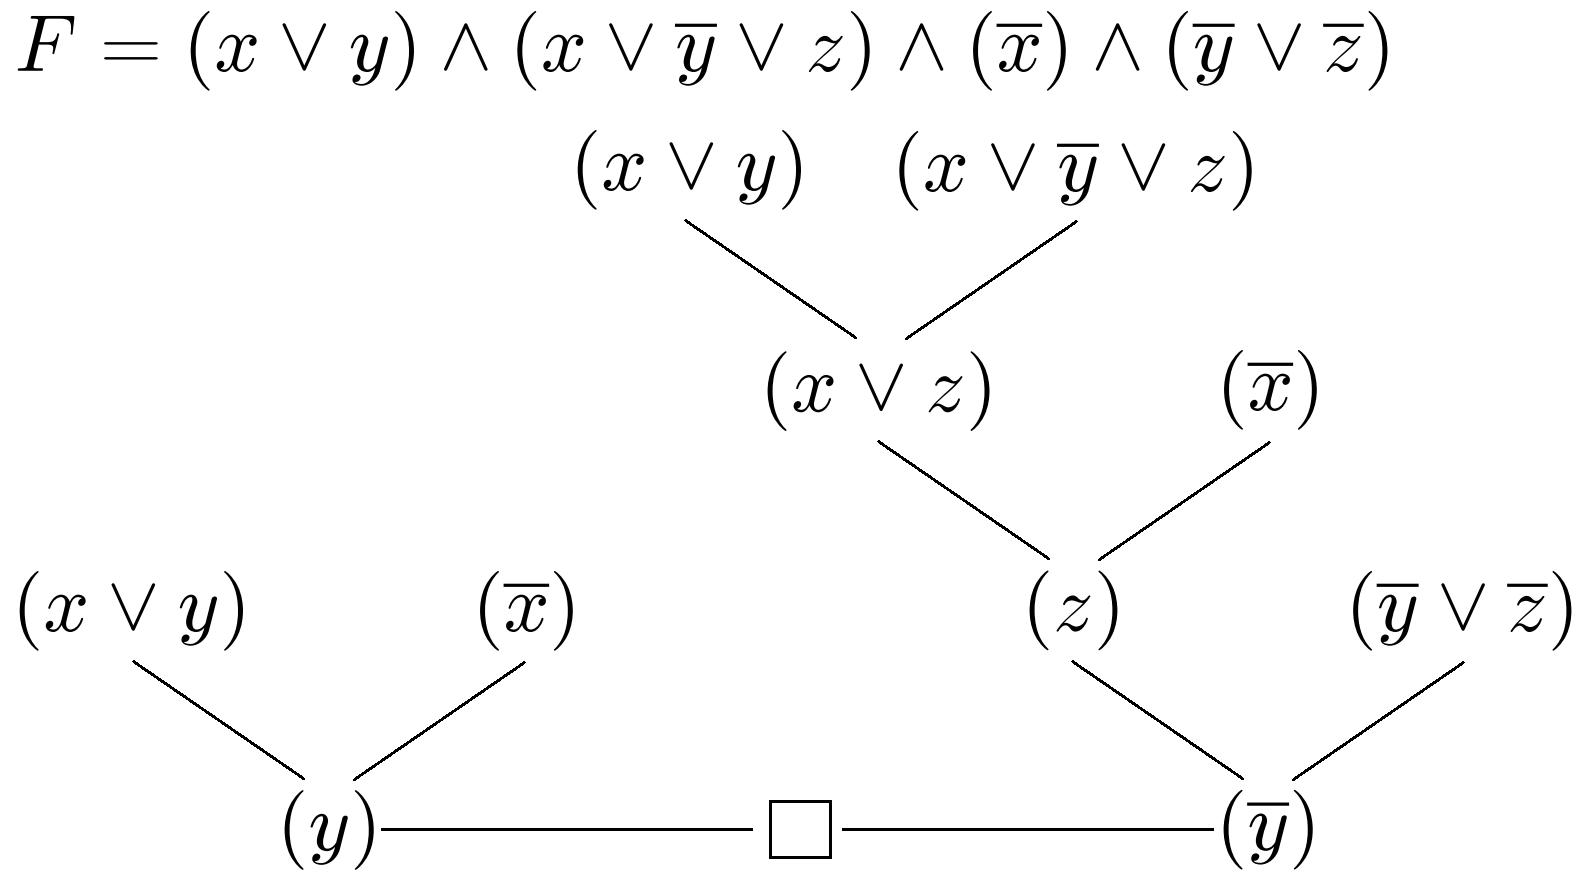
\includegraphics{img/res-beweis.png}
\end{figure}

\end{frame}

\begin{frame}{Indizien}{Resolution als Indiz für coNP $\neq$ NP}

\begin{itemize}
\itemsep1pt\parskip0pt\parsep0pt
\item
  1985 bewies Haken eine untere Schranke für die Größe des
  Resolutionsbeweises für das Taubenschlagprinzip
\item
  Diese ist $(1.49^{0.01})^n \approx (1,004)^n$ und unabhängig vom
  gewählten Algorithmus
\item
  Aufbauend auf Hakens Beweis wurden exponentielle untere Schranken auch
  für andere Probleme gezeigt

  \begin{itemize}
  \itemsep1pt\parskip0pt\parsep0pt
  \item
    mittels Resolution ist coNP = NP nicht beweisbar
  \item[$\Rightarrow$] Indiz für coNP $\neq$ NP
  \end{itemize}
\end{itemize}

\end{frame}

\section{Implikationen}\label{implikationen}

\begin{frame}{Implikationen}{Philosophisch}

\begin{itemize}
\itemsep1pt\parskip0pt\parsep0pt
\item
  In den Naturwissenschaften wären Hypothesen mit vergleichbarer
  Faktenlage als Theorien anerkannt.

  \begin{itemize}
  \itemsep1pt\parskip0pt\parsep0pt
  \item
    „nur`` ein Problem weil Informatik eine Strukturwissenschaft ist
  \end{itemize}
\item
  Folgen oft völlig unintuitiv:

  \begin{itemize}
  \itemsep1pt\parskip0pt\parsep0pt
  \item
    Warum sollte es keine Suchprobleme geben, die sich nicht besser als
    mit brute-force lösen lassen?
  \item
    Insbesondere bei nichtdeterministischen TMs: Polyzeitreduktion
    praktisch nicht vorstellbar.
  \item
    Alle Probleme in NP, die nicht auch in leichteren Klassen als P liegen, vergleichbar
    schwer, es gäbe keine Klasse NPI
  \end{itemize}
\end{itemize}

\end{frame}

\begin{frame}{Implikationen}{Kryptographisch}

\begin{itemize}
\itemsep1pt\parskip0pt\parsep0pt
\item
  Nicht \textbf{zwingend} katastrophal

  \begin{itemize}
  \itemsep1pt\parskip0pt\parsep0pt
  \item
    Feste aber große Exponenten reichen vermutlich auch:
    $2^{512} \ll 512^{100}$
  \item
    Heutige Krypto meist nicht NP-vollständig (Faktorisierung in NPI
    vermutet)
  \item
    Quantencomputer sind hier eine \textbf{viel} realere Bedrohung.\\
    ($\rightarrow$ Shor-Algorithmus)
  \end{itemize}
\item
  Andererseits: Passwort raten, leicht gemacht?

  \begin{itemize}
  \itemsep1pt\parskip0pt\parsep0pt
  \item
    Gibt es ein Passphrase der Länge $\le n$ die diese Datei
    entschlüsselt? $\in$ NP
  \end{itemize}
\end{itemize}

\end{frame}

\begin{frame}{Implikationen}{coNP $\stackrel{?}{=}$ NP}

\begin{itemize}
\itemsep1pt\parskip0pt\parsep0pt
\item
  Aus P = NP folgt automatisch coNP = NP

  \begin{itemize}
  \itemsep1pt\parskip0pt\parsep0pt
  \item
    Umkehrung gilt nicht automatisch
  \end{itemize}
\item
  Allerding folgt aus coNP $\neq$ NP automatisch P $\neq$ NP:

  \begin{itemize}
  \itemsep1pt\parskip0pt\parsep0pt
  \item
    man wählt ein NP-vollständiges Problem $L$
  \item
    das Komplement $\overline{L}$ von $L$ liegt laut Definition in coNP
  \item
    würde P = NP gelten, gilt $L \in$ P
  \item
    da P unter Komplementbildung abgeschlossen ist gilt
    $\overline{L} \in$ P
  \item
    da gilt P = NP gilt $\overline{L} \in$ NP
  \item
    daraus würde folgen coNP = NP was ein Wiederspruch ist
  \end{itemize}
\end{itemize}

\end{frame}


\section[Umgang]{Umgang mit NP-vollständigen Problemen}

\begin{frame}{Umgang mit NP-vollständigen Problemen}

\begin{figure}[htbp]
\centering

\includegraphics{img/dont_panic.png}
\end{figure}

\end{frame}

\begin{frame}{Umgang mit NP-vollständigen Problemen}

\begin{itemize}
\itemsep1pt\parskip0pt\parsep0pt
\item
  Exisitieren vielleicht gute Näherungslösungen?
\item
  Ist der Worst-Case wirklich wahrscheinlich?
\item
  Ist $n$ wirklich so groß, dass NP-Vollständigkeit ein Problem
  darstellt?
\end{itemize}

\end{frame}

\begin{frame}{Umgang mit NP-vollständigen Problemen}

\begin{itemize}
\itemsep1pt\parskip0pt\parsep0pt
\item
  Gibt es vielleicht bessere, nicht NP-schwere Modelierungen?
\end{itemize}

\begin{figure}[htbp]
\centering
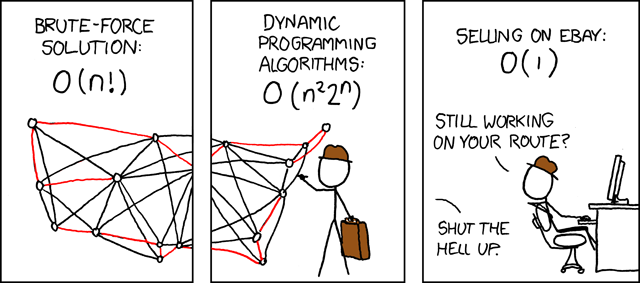
\includegraphics{img/travelling_salesman_problem.png}
\end{figure}

\end{frame}

\section{Zusammenfassung}\label{zusammenfassung}

\begin{frame}{Zusammenfassung}

\begin{itemize}
\itemsep1pt\parskip0pt\parsep0pt
\item
  Alle NP-Probleme können in Polyzeit auf NP-vollständigen Probleme
  reduziert werden.
\item
  Wichtige Beispiele für NP-vollständige Probleme sind SAT, 3SAT,
  INDSET, 0/1-PROG und TSP
\item
  Analoge Probleme existieren auch in diversen anderen Klassen
\item
  P$\neq$NP ist zwar \emph{unbewiesen} aber es gibt sehr gute
  \emph{Indizien} dafür
\item
  Die Implikationen von P=NP sind gravierend, aber nicht zwingend
  katastrophal
\item
  In der Realität sind NP-vollständige Probleme bisweilen gut zu
  meistern
\end{itemize}

\end{frame}

\section{Quellenangaben}\label{quellenangaben}

\begin{frame}{Quellen}{Literatur}
\begin{itemize}
	\item „Aussagenlogik: Deduktion und Algorithmen“ von Hans Kleine Büning und Theodor Lettmann
		%\url{https://books.google.de/books?id=6ZGoBgAAQBAJ&pg=PA150}
	\item „Computational Complexity: A Modern Approach“ von Sanjeev Arora und Boaz Barak
\end{itemize}
\end{frame}

\begin{frame}{Quellen}{Online}

\begin{itemize}
	\item \url{http://de.wikipedia.org/wiki/}
		\begin{itemize}
			\item \url{AKS-Primzahltest}
			\item \url{Satz\_von\_Ladner}
			\item \url{NP-intermediate}
		\end{itemize}
	\item \url{https://complexityzoo.uwaterloo.ca/}
		\begin{itemize}
			\item \url{Complexity\_Zoo:B\#bqp}
			\item \url{Complexity\_Zoo:B\#bpp}
			\item \url{Complexity\_Zoo:C\#conp}
			\item \url{Complexity\_Zoo:P\#p}
			\item \url{Complexity\_Zoo:Q\#qma}
		\end{itemize}
\end{itemize}
\end{frame}

\begin{frame}{Quellen}{Online}
\begin{itemize}
	\item \url{https://homepages.uni-tuebingen.de//student/monika.gehweiler/Applets/html/resolutionIndex.html}
	\item \url{http://www.ti.inf.ethz.ch/ew/lehre/extremal04/raemy.pdf}
	\item \url{http://www.cs.cmu.edu/afs/cs.cmu.edu/academic/class/46927-f97/slides/Lec4/sld033.htm}
	\item \url{http://www.cosy.sbg.ac.at/~held/teaching/wiss\_arbeiten/slides\_02-03/kmrr.pdf}
	\item \url{http://hackvalue.de/files/tsp.pdf}
	\item \url{http://www.scottaaronson.com/blog/?p=1720}
\end{itemize}
\end{frame}

\begin{frame}{Quellen}{Abbildungen}
\begin{itemize}
	\item Motivations-Comics: „Computers and Intractability -- A Guide to the Theory of NP-Completeness“ von Michael R. Garey und David S. Johnson
	\item Lego-Turingmaschine: \url{http://www.legoturingmachine.org}
	\item Stephen Cook (CC-BY-SA 3.0, Jiří Janíček):
		\url{https://commons.wikimedia.org/wiki/File:Prof.Cook.jpg}
	\item Leonid Levin (CC-BY-SA 3.0, Sergio01):
		\url{https://commons.wikimedia.org/wiki/File:LeonidLevin2010.jpg}
\end{itemize}
\end{frame}

\begin{frame}{Quellen}{Abbildungen}
\begin{itemize}
	\item TSP-Karte (CC-BY-SA 3.0): \url{http://commons.wikimedia.org/wiki/File:Deutschland_topo.png}
	\item „My Hobby“ (CC-BY-NC 2.5, Randall Munroe): \url{https://xkcd.com/287/}
	\item „Don't Panic“: \url{http://everfalling.deviantart.com/art/DON-T-PANIC-15975789}
	\item „Traveling Salesman“ (CC-BY-NC 2.5, Randall Munroe): \url{https://xkcd.com/399/}
\end{itemize}
\end{frame}

\end{document}
